% Define a classe do documento
\documentclass[a4paper,12pt]{article}

% Inclusão de pacotes
\usepackage[brazil]{babel}
\usepackage[utf8]{inputenc}
\usepackage[T1]{fontenc}

% Inclusão de figuras
\usepackage{graphicx}
\usepackage{subfig}

% Inclusão do citeonline
\usepackage[sort]{cite}

\usepackage{lipsum}

\usepackage[alf]{abntex2cite}

% Definição de variáveis
\title{Aula02 - \LaTeX}
\author{Chauã Queirolo \\ Fulano de tal}
\date{}

% Documento principal
\begin{document}

\maketitle
\tableofcontents

\begin{abstract}
    \lipsum[2]
\end{abstract}


\section{Introdução}

\lipsum[2]

\section{Metodologia}
\lipsum[2]

A Seção~\ref{sec:algo1} apresenta a implementação do algoritmo de busca binária. As Seções~\ref{sec:algo2}~e~\ref{sec:algo-extra} apresentam os algoritmos de ordenação e inserção, respectivamente.

\subsection{Algoritmo 1}
\label{sec:algo1}
\lipsum[2]

A Figura~\ref{fig:grafico-barras} apresenta os resultados da pesquisa de nível de serviço do ano de 2022.

% Exemplo de figura
\begin{figure}[ht]
    \centering
    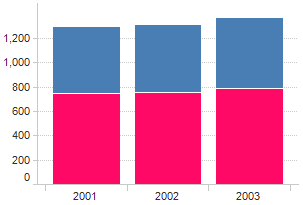
\includegraphics[width=8cm]{img/grafico-barras.png}
    \caption{Exemplo de gráfico de barras.}
    \label{fig:grafico-barras}
\end{figure}


\subsection{Algoritmo 2}
\label{sec:algo2}

\lipsum[4]

A Tabela~\ref{tab:exemplo} apresenta os resultados obtidos.

\begin{table}[h]
    \centering
    \caption{Exemplo de tabela.}
    \label{tab:exemplo}  
    \begin{tabular}{|l||c|p{4cm}|}
       \hline
       \textbf{C1} & \textbf{C2} & \textbf{C3} \\ \hline \hline
        A          & B           & C           \\ \hline
        D          & E           & F           \\ \hline
   \end{tabular} 
\end{table}



\subsection{Algoritmo extra}
\label{sec:algo-extra}

\lipsum[4]

% Exemplo de subfigura
\begin{figure}[ht]
    \centering
    \subfloat[][Imagem original]{
        \label{fig:parte1}   
        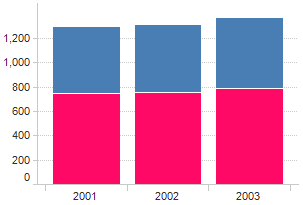
\includegraphics[width=3cm]{img/grafico-barras.png}
    }
    \subfloat[][Imagem alterada]{
        \label{fig:parte2}   
        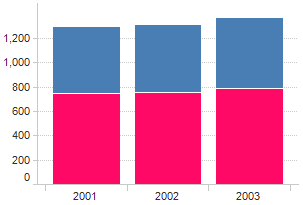
\includegraphics[width=3cm]{img/grafico-barras.png}
    }

    \subfloat[][]{
        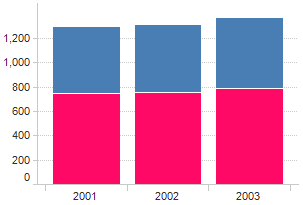
\includegraphics[width=3cm]{img/grafico-barras.png}
    }
    \subfloat[][]{
        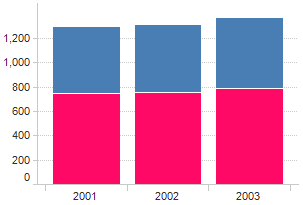
\includegraphics[width=3cm]{img/grafico-barras.png}
    }

    \caption{Exemplo de gráfico de barras.}
    \label{fig:grafico-barras-2}
\end{figure}

\lipsum[4]

A Equação~\ref{eq:peppers} mostra a fórmula de Peppers, onde, $r$ é o raio. A variável $x$ e $y$ são invariáveis.

% Ambiente permite a referência
\begin{equation}
\label{eq:peppers}
A = \frac{\pi r^2}{2} = \frac{1}{2} \pi r^2   
\end{equation}

\lipsum[4]

$$
A = \frac{\pi r^2}{2} = \frac{1}{2} \pi r^2   
$$

\lipsum[4]

Os métodos utilizados não forma muito precisos~\cite{ref:darwin1872, ref:ross2006}.
De acordo com~\citeonline{ref:ross2006}, blá blá blá.


\section{Conclusão}

\lipsum[4]

\bibliography{referencias}



\end{document}
